\documentclass{report}
\usepackage[utf8]{inputenc}
\usepackage{booktabs}
\usepackage{graphicx}
\usepackage[english]{babel}
\usepackage{hyperref}
\usepackage{enumitem}
\usepackage[backend=biber,style=verbose-trad2, citestyle=numeric]{biblatex}
\usepackage{listings, xcolor}
\usepackage{tikz}
\usepackage{aeguill}
\usepackage[yyyymmdd]{datetime}
\renewcommand{\labelenumii}{\arabic{enumi}.\arabic{enumii}}
\renewcommand{\labelenumiii}{\arabic{enumi}.\arabic{enumii}.\arabic{enumiii}}
\renewcommand{\labelenumiv}{\arabic{enumi}.\arabic{enumii}.\arabic{enumiii}.\arabic{enumiv}}
\renewcommand{\dateseparator}{.}
\addbibresource{Citations/a-5.bib}
\lstset{
tabsize = 4, %% set tab space width
showstringspaces = false, %% prevent space marking in strings, string is defined as the text that is generally printed directly to the console
numbers = left, %% display line numbers on the left
commentstyle = \color{green}, %% set comment color
keywordstyle = \color{blue}, %% set keyword color
stringstyle = \color{red}, %% set string color
rulecolor = \color{black}, %% set frame color to avoid being affected by text color
basicstyle = \small \ttfamily , %% set listing font and size
breaklines = true, %% enable line breaking
numberstyle = \tiny,
}
\newlist{parlist}{enumerate}{1}
\setlist[parlist]{label=(\alph*),wide=0pt,topsep=0pt}


\begin{document}
\begin{center}
    
\end{center}
    \begin{figure}[htb]
            \centering
\includegraphics[width=.5\textwidth]{Immagini/FUlogo.png}
    \end{figure}
    

 {\centering\scshape\LARGE\bfseries Aufgabe 6
    \begin{center}
       Nathan Ritter  \\ 5566519 \\
       Lorenzo Tecchia \\ 5581906  \\ \today
    \end{center}}


    \newpage
    
    \tableofcontents
    \listoffigures
    
    \chapter{Task 1}
\begin{parlist}
	\item Use cases describe interactions between users and a system using a graphical model and a structured text. A use case indentifies the actors involved in an interaction and names the type of interaction. Additional information can be added in order to describe the interaction with the system. Those additional information can be a textual description or one or more models such as the UML sequence diagram or the state charts.
	\item 
		\begin{enumerate}
			\item We identified these criteria for the product view:
				\begin{itemize}
					\item Hold Functional Requirements in an easy to read, easy to track text format.
					\item Represents the goal of an interaction between an actor and the system. The goal represents a meaningful and measurable objective for the actor.
					\item Records a set of paths (scenarios) that traverse an actor from a trigger event (start of the use case) to the goal (success scenarios).
					\item Records a set of scenarios that traverse an actor from a trigger event toward a goal but fall short of the goal (failure scenarios).
					\item Are multi-level: one use case can use/extent the functionality of another. \cite{cockburnComingSoon}
				\end{itemize}
			\item We identified these criteria for the process view:	
				\begin{itemize}
					\item The sentence shows the intent of the actor, not their particular movements in accomplishing that intent (semantics, not dialog).\cite{cockburnComingSoon}
					\item All the action depicted by the use cases should have neutrality inside their representation. 
					\item The sentence shows the process moving distinctly forward. \cite{Adolph:2003aa}
					\item Since we're not gonna describe the interface with which the actors interact(e.g. the GUI of a software) but instead the control of action that is exchanged from one actor to another(e.g. data passes from actor B to actor A or vice versa).\cite{Sommerville:2004aa}
					\item Mentioning the timing is optional.
				\end{itemize}			
		\end{enumerate}
	%\item A scenario starts with an outline of the interaction. During the elicitation process, details are added to create a complete description of that interaction. It can include a description of what the system and user expect when the scenario starts, a description of the normal flow of the events in the scenario, a description of what can go wrong and how resulting problems can be handled, information about other activities that might be going on at the same time, a description of the system state when the scenario ends.\cite{Sommerville:2004aa}\\ So from the statements from above we can clearly see the difference: use cases show "how the ball is passed", in particular how the control of the system gets passed from one actor to another, and its depiction it's as precise and not-ambiguous as it is necessary for the determined use case. As said the timing of all of these action in use cases is not necessary.
	\item The difference between a usecase and a scenario is that a scenario is a concrete realisation of a use case, so there are no variations only one flow of events and concrete Data etc. A scenario represents one particular example situation with these values etc. where as a use case more of describes a class/type of situation. 
\end{parlist}

    \chapter{Task 2}
\begin{parlist}
	\item Solution:
	\begin{figure}[hbt]
		\makebox[\textwidth][c]	{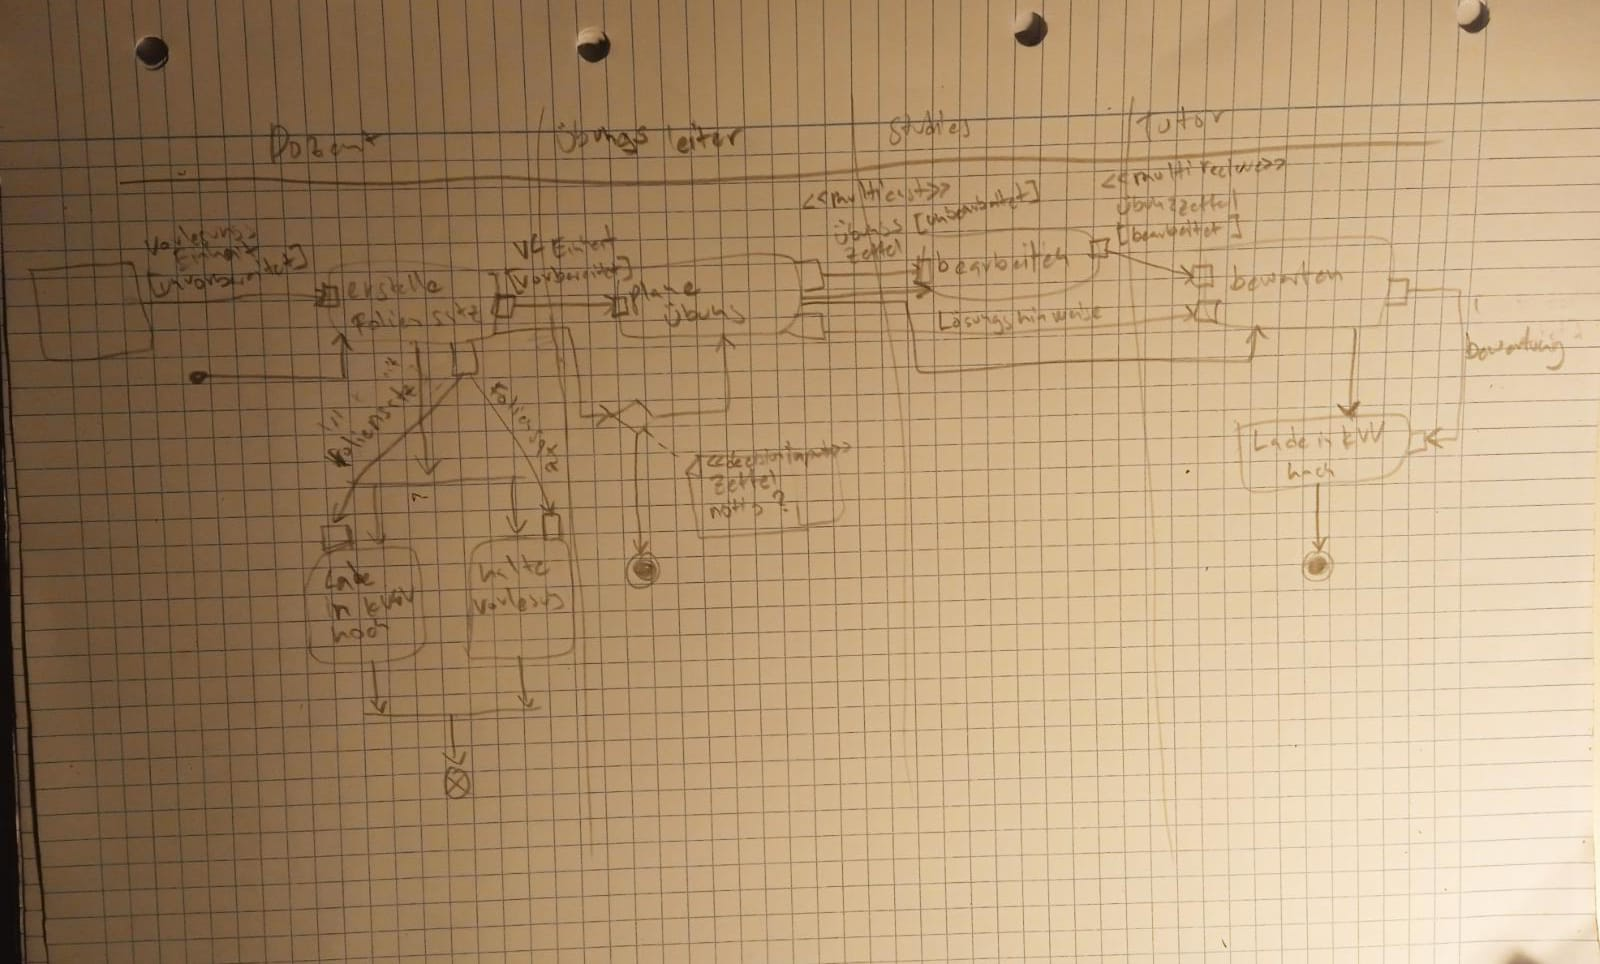
\includegraphics[width=1.7\textwidth]{Immagini/WhatsApp Image 2023-05-27 at 9.21.26 PM.jpeg}}
  \caption{Activity Diagram}
  \label{fig:ActDia}
\end{figure}

\end{parlist}
    

    \chapter{Chapter 3}

    
    
    \printbibliography
    
\end{document}